\documentclass[12pt]{article}
\usepackage[margin=1.5cm, includehead, includefoot, headsep=10pt, footskip=30pt]{geometry}

% Load TikZ package
\usepackage{tikz}
\usetikzlibrary{trees}

\begin{document}

\title{Report on improvement in BST}
\author{Zhu Kongyang}
\maketitle

\section{Remark}
Thx to GPT for helping with the TikZ drawn BST diagrams!

\section{Unsolved Problems}
Again my latex failed n' that's y I'm using English. I'm upgrading my computer, and I'll retry my debian cuz WSL's so STUPID. But the document compiled well on my classmate's ubuntu, so I'm not sure what the problem is. I'll try to fix it.

\section{PS}
I didn't delete the Chinese version. The name is report\_chi.tex. U can check it out.

\section{Implementation of the Modified remove Function}
The detachMin function is used to find and detach the minimum node in a given subtree. The modified `remove` function handles node deletion in the following three scenarios:

\begin{itemize}
  \item 1: The node to be deleted has no children. The node is simply deleted.
  \item 2: The node to be deleted has one child. The node is deleted and replaced by its child.
  \item 3: The node to be deleted has two children. Find the minimum node in the right subtree, copy its value to the current node, and then delete the minimum node in the right subtree.
\end{itemize}

\section{Presentation and Analysis of Test Output Results}

The initial tree structure is as follows:

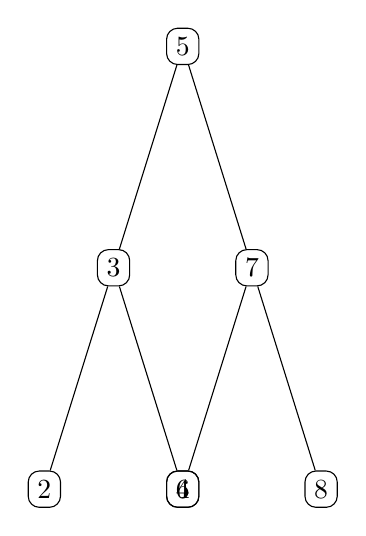
\begin{tikzpicture}[sibling distance=5em, level distance=8em, 
  every node/.style = {shape=rectangle, rounded corners, draw, align=center}]
  \node {5}
    child {node {3}
      child {node {2}}
      child {node {4}}
    }
    child {node {7}
      child {node {6}}
      child {node {8}}
    };
\end{tikzpicture}

After removing element 3:

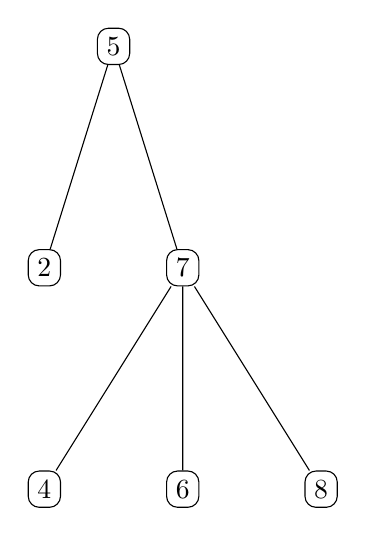
\begin{tikzpicture}[sibling distance=5em, level distance=8em, 
  every node/.style = {shape=rectangle, rounded corners, draw, align=center}]
  \node {5}
    child {node {2}}
    child {node {7}
      child {node {4}}
      child {node {6}}
      child {node {8}}
    };
\end{tikzpicture}

After removing element 5:

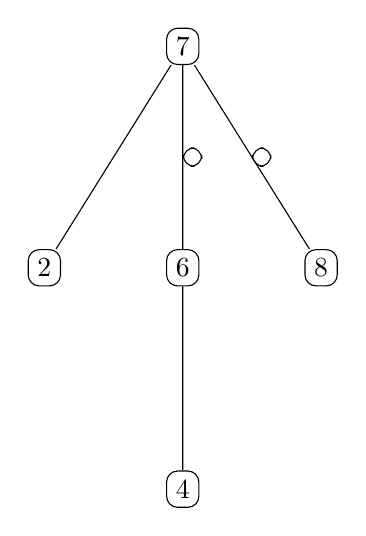
\begin{tikzpicture}[sibling distance=5em, level distance=8em, 
  every node/.style = {shape=rectangle, rounded corners, draw, align=center}]
  \node {7}
    child {node {2}}
    child {node {6}
      child {node {4}}
      edge from parent node [right] {}}
    child {node {8} edge from parent node [right] {}};
\end{tikzpicture}

After removing element 8:

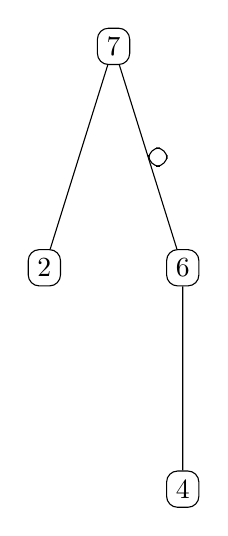
\begin{tikzpicture}[sibling distance=5em, level distance=8em, 
  every node/.style = {shape=rectangle, rounded corners, draw, align=center}]
  \node {7}
    child {node {2}}
    child {node {6}
      child {node {4}}
      edge from parent node [right] {}};
\end{tikzpicture}

From the test results, it can be seen that after each deletion operation, the left subtree of any node only contains values less than that node, and the right subtree only contains values greater than that node. This indicates that the modified `remove` function is correct.

\end{document}